\chapter{四波混频}
\label{ch:FWM}

根据公式~\ref{eq:average_power}计算出的单一频率光的平均功率在一段时间内是恒定的。如果存在两个频率,它们之间的干涉会导致平均功率随时间正弦变化。由于 $\gamma\neq0$ 意味着折射率取决于功率,因此在非线性介质中同时存在两个频率的光意味着相位将被正弦调制。这种效应会产生新的频率成分,被称为 “四波混频”(FWM)。



\section{电相位调制}

要了解四波混频,首先要考虑将连续波激光信号发射到商用相位调制器中,并由函数发生器发出的正弦电信号驱动。可视化效果见图 ~\ref{fig:PM},实验演示见 \href{https://youtu.be/j8It3to54AQ}{此视频}。输出端的信号由以下公式给出

\begin{align}
    \label{eq:phase_modulator}
    \E_{out}&=\E_{in}\exp\left(i\Phi\cos(\omega_dT), \right)
\end{align}

其中,$\Phi$ 是调制器传递的最大相移,$\omega_d$ 是调制频率。关于这种调制对 $\E_{out}$ 实部的影响,请参见 \href{https://www.desmos.com/calculator/vcreo1gs2q}{此交互式图表}。使用所谓的 “雅各比-安格尔展开式”~\cite{NIST_JA_expansion},公式~\ref{eq:phase_modulator}中复数指数内的余弦函数可以写为

\begin{align}
\label{eq:JA}
    \exp\left(i\Phi\cos(\omega_dT)\right) &= \sum_{n=-\infty}^{\infty}i^n J_n(\Phi) \exp\left(in\omega_dT\right),
\end{align}
其中,$J_n(\Phi)$ 是$n^{th}$ 阶贝塞尔函数的第 1 种。简而言之,公式 ~\ref{eq:JA} 表明正弦相位调制会产生间隔为 $\omega_d$ 的新的离散频率成分,其相对功率取决于调制幅度 $\Phi$。还请注意,将公式 ~\ref{eq:chirp_definition}应用于公式 ~\ref{eq:phase_modulator}显示,正弦调制会随着时间改变瞬时频率,改变幅度为 $\Phi\omega_d\sin(\omega_dT)$,这进一步表明相位调制会改变入射光的颜色。
\begin{figure}
    \centering
    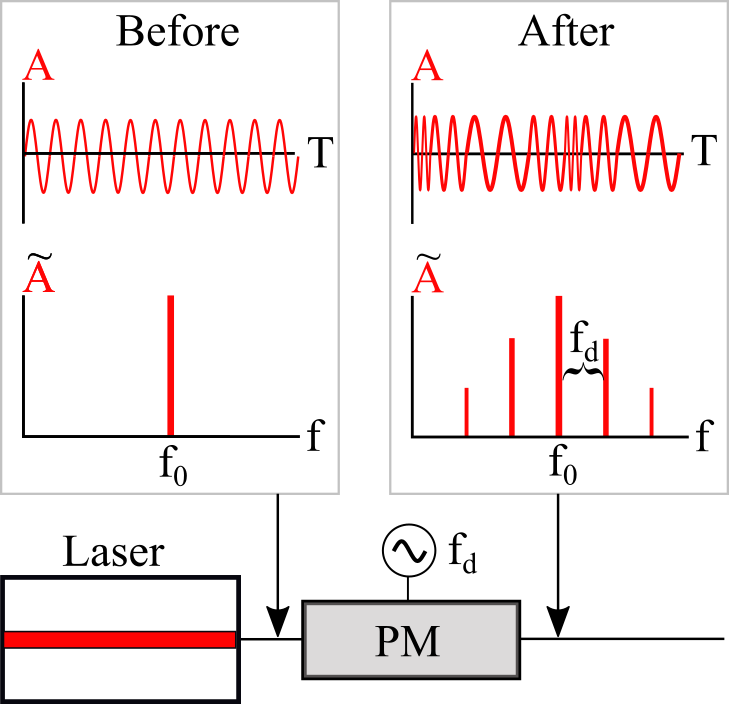
\includegraphics[width=1\linewidth]{figures/PhaseModulator.png}
    \caption{正弦波相位调制对连续波光信号的影响示意图。在进入调制器之前,只有一个激光频率。进入调制器后,根据公式~\ref{eq:JA},光相位在时域中的交替前进和延迟相当于引入了新的频率成分。}
    \label{fig:PM}
\end{figure}

\section{非线性相移}
\label{sec:sidebands}

以下的 FWM 建模方法受到~\cite{Boskovic_Original_Kerr_Effect}中最初提出的方法的启发。考虑公式 ~\ref{eq:SPM_applied},并假设场 $\A(0,T)$ 可以写成两个连续波信号的和,这两个连续波信号的平均功率分别为 $P_a$ 和 $P_b$,频率间隔为 $\Delta\omega$ 。
\begin{align}
    \label{eq:FWM_input}
    \A(0,T)&= \sqrt{P_a}e^{-i\frac{\Delta\omega}{2}T}+\sqrt{P_b}e^{i\frac{\Delta\omega}{2}T}.
\end{align}
当信号由两个持续时间有限的脉冲组成时,连续波假设是一个近似值,当 $\omega_d$ 大于脉冲的带宽时,连续波假设是有效的。非线性介质末端的场为
\begin{align}
    \A(L,T) &= \A(0,T)\exp\left(i\gamma L [P_a+P_b+2\sqrt{P_aP_b}\cos(\omega_dT)] \right) \\ \nonumber
    &= \A(0,T)\exp\left(i\gamma L [P_a+P_b]\right)\exp\left(i2\gamma L\sqrt{P_aP_b}\cos(\omega_dT) \right)\\ \nonumber
    \A(L,T)Q^{-1}&= \A(0,T)\exp\left(i2\gamma L\sqrt{P_aP_b}\cos(\omega_dT) \right)\\ \nonumber
    \A(L,T)Q^{-1}&= \A(0,T)\exp\left(i\phi_{NL}\cos(\omega_dT) \right),
\end{align}
其中,为方便起见,时间无关因子 $Q=\exp(i\gamma L [P_a+P_b])$暂时移至等式左侧。应用公式 ~\ref{eq:JA} 得出
\begin{align}
    \A(L,T)Q^{-1}&= \A(0,T)\sum_{n=-\infty}^{\infty}i^nJ_n(\phi_{NL})e^{in\omega_dT} \\ \nonumber
    &=\left(\sqrt{P_a}e^{-i\frac{\Delta\omega}{2}T}+\sqrt{P_b}e^{i\frac{\Delta\omega}{2}T}\right)\sum_{n=-\infty}^{\infty}i^nJ_n(\phi_{NL})e^{in\omega_dT} \\ \nonumber
    &=\sqrt{P_a}\sum_{m=-\infty}^{\infty}i^mJ_m(\phi_{NL})e^{i\left(m-\frac{1}{2}\right)\omega_dT}+...\\ \nonumber & \quad\quad\quad\quad\quad\sqrt{P_b}\sum_{k=-\infty}^{\infty}i^kJ_k(\phi_{NL})e^{i\left(k+\frac{1}{2}\right)\omega_dT}.
\end{align}

请注意,由于 $\A(0,T)$ 中的两个复指数导致第一个和中 $m=1$ 所对应的频率与第二个和中 $k=1$ 所对应的频率不同,因此最初以 $n$ 为索引的无限和被拆分为两个以 $m$ 和 $k$ 为索引的无限和。要重新组合这两个和,使用 $m=k+1$ 并得到
\begin{align}
\label{eq:re_index}
    \A(L,T)Q^{-1}&=\sqrt{P_a}\sum_{k=-\infty}^{\infty}i^{k+1}J_{k+1}(\phi_{NL})e^{i\left(k+\frac{1}{2}\right)\omega_dT}+...\\ \nonumber & \quad\quad\quad\quad\quad\sqrt{P_b}\sum_{k=-\infty}^{\infty}i^kJ_k(\phi_{NL})e^{i\left(k+\frac{1}{2}\right)\omega_dT} \\ \nonumber
    &= \sum_{n=-\infty}^{\infty} i^n\left[i\sqrt{P_a}J_{n+1}\left(\phi_{NL}\right)+\sqrt{P_b}J_n\left(\phi_{NL}\right)\right]e^{i\omega_d\left(n+\frac{1}{2}\right)T}.
\end{align}
最后,把 $Q$ 移到公式 ~\ref{eq:re_index} 的右边,得到
\begin{align}
\label{eq:FWM_general}
    \A(L,T)&=\sum_{n=-\infty}^{\infty} i^n\left[i\sqrt{P_a}J_{n+1}\left(2\gamma L\sqrt{P_aP_b}\right)+\sqrt{P_b}J_n\left(2\gamma L\sqrt{P_aP_b}\right)\right]e^{i\omega_d\left(n+\frac{1}{2}\right)T+i\gamma L[P_a+P_b]}.
\end{align}

在公式 ~\ref{eq:FWM_general}中,$n=-1$ 的频率分量将位于 $-\omega_d/2$,而 $n=0$ 的频率分量将位于 $+\omega_d/2$,与公式 ~\ref{eq:FWM_input}中的原始两个频率相对应。$n^{th}$ 阶边带的平均功率为
\begin{align}
\label{eq:sideband_power}
    |\A_n(L,T)|^2 &= P_aJ^2_{n+1}\left(2\gamma L \sqrt{P_aP_b}\right)+P_bJ^2_{n}\left(2\gamma L \sqrt{P_aP_b}\right).
\end{align}
请参见图(fig:FWM)a) 和 b),这是针对不同的 $2\gamma L \sqrt{P_aP_b}$ 值对边带功率进行的数值模拟。请参见图 ~\ref{fig:FWM} c) ,比较数值计算的边带功率和公式 ~\ref{eq:sideband_power}预测的功率。假设 $P_a\ll P_b$ 和 $2\gamma L\sqrt{P_aP_b}<\sqrt{1+n}$ 且 $n>0$ 可以得到

\begin{align}
\label{eq:sideband_approx}
    |\A_n(L,T)|^2 &\approx P_b\frac{(\gamma^2 L^2P_aP_b)^{n}}{n!^2},
\end{align}
since
\begin{align}
\label{eq:Bessel_approx}
    J_n(x)&\approx \frac{1}{n!}\left(\frac{x}{2}\right)^n
\end{align}

为贝塞尔函数中的参数。请参见图~ref{fig:FWM} d) 以了解公式~\ref{eq:sideband_approx}预测的缩放行为。与低阶边带相比,高阶边带的功率对输入功率的变化更为敏感,这一事实对于各种全光信号处理技术非常有用~\cite{my_thesis,BenoitPhD,YangLuPhD}。请参阅(\href{https://youtu.be/0SXPvO89jto}{本教程视频},了解将色散因素考虑在内的全波调制建模的不同方法。参见 \href{https://youtu.be/gsa9hrCbnqI}{这段视频},了解四波混频的实验演示。
\begin{figure}
    \centering
    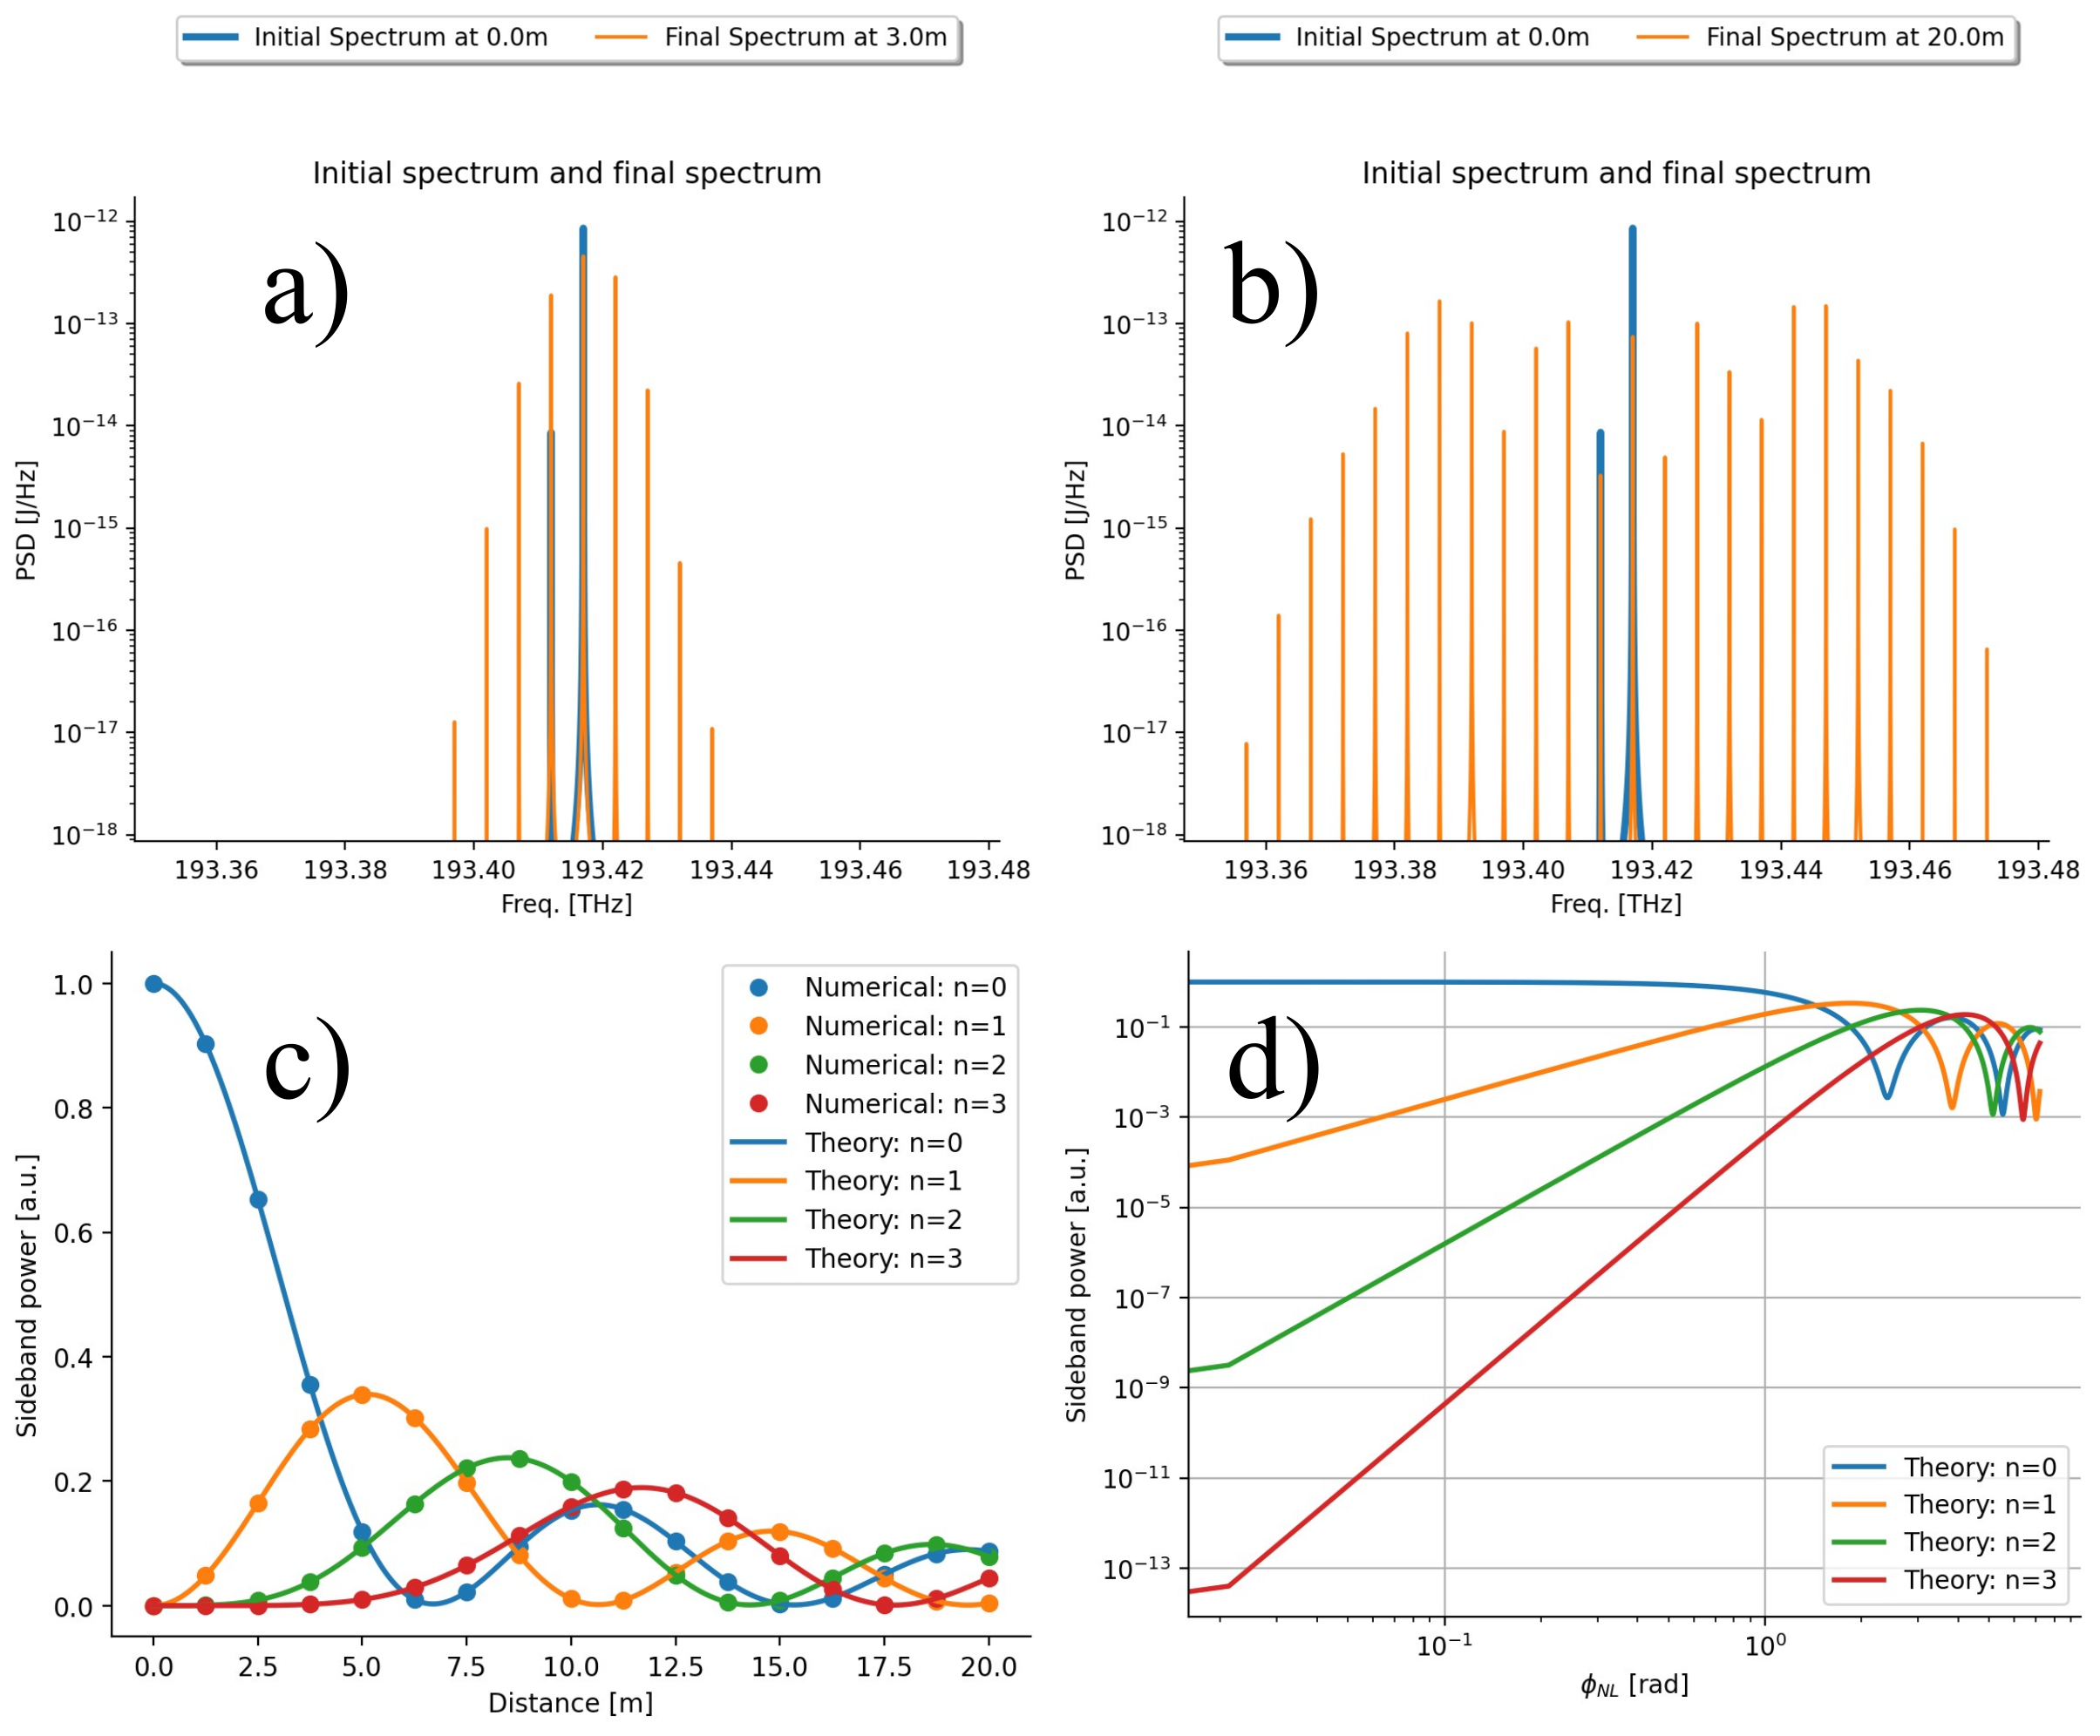
\includegraphics[width=1.0\linewidth]{figures/FWM_combined.png}
    \caption{a) 当两个相距 5~GHz 的频率($P_b=100P_a$)在介质中传播时,数值计算的初始和最终频谱,其中 $\phi_{NL}=2\gamma L\sqrt{P_aP_b}=1.08$~rad. b) 与 a) 相同,但 $\phi_{NL}=2\gamma L\sqrt{P_aP_b}=7.2$~rad. c) 根据数值模拟和公式~\ref{eq:sideband_power},边带功率归一化为 $P_b$ 的比较。 d) 与 c) 类似,但绘制了双对数刻度与 $\phi_{NL}$ 的关系图,以展示公式~\ref{eq:sideband_approx}预测的缩放行为。这些图是使用 \href{https://colab.research.google.com/drive/1l054EDg-50aK5GORN_md4_-tlFy4jwC5?usp=sharing}{这个交互式笔记本}生成的,我们鼓励读者尝试使用。   }
    \label{fig:FWM}
\end{figure} 

\section{交叉相位调制(XPM)}
\label{Sec:XPM}
第~\ref{ch:SPM}章指出,非线性介质中单频光场的相位与该场的平均功率呈线性增长。当存在两个频率时,一个频率分量的相位与其自身的平均功率和另一个频率分量的平均功率的函数关系可以通过公式~\ref{eq:FWM_general}计算出来。选择 $n=0$ 分量可得到
\begin{align}
    \phi_0 &= \frac{\omega_d}{2}T+\gamma L [P_a+P_b]+\theta_0,
\end{align}
这里,
\begin{align}
\label{eq:theta}
    \theta_0 &= arg\left( i\sqrt{P_a}J_{1}\left(2\gamma L\sqrt{P_aP_b}\right)+\sqrt{P_b}J_0\left(2\gamma L\sqrt{P_aP_b}\right) \right) \\ \nonumber
    &= \arctan\left(\frac{\sqrt{P_a}J_{1}\left(2\gamma L\sqrt{P_aP_b}\right)}{\sqrt{P_b}J_0\left(2\gamma L\sqrt{P_aP_b}\right) } \right).
\end{align}
使用公式~\ref{eq:Bessel_approx}可以将公式~\ref{eq:theta}写成
\begin{align}
    \theta_0 &\approx\arctan\left(\frac{\sqrt{P_a}\gamma L\sqrt{P_aP_b}}{\sqrt{P_b} } \right) \\ \nonumber
    &\approx\arctan\left(\gamma LP_a\right) \\ \nonumber
    &\approx \gamma LP_a.
\end{align}
因此,$n=0$ 频率分量的相位为
\begin{align}
    \label{eq:XPM}
    \phi_0 &\approx \frac{\omega_d}{2}T+\gamma L [P_a+P_b]+\gamma LP_a \\ \nonumber
    &=\frac{\omega_d}{2}T+\gamma L [2P_a+P_b].
\end{align}
请注意,$n=0$ 为 $+\omega_d/2$ 处的频率,该频率最初的平均功率为 $P_b$。因此,式 ~\ref{eq:XPM} 中包含 $P_b$ 的项对应于 SPM 的影响,而包含 $P_a$ 的项对应于所谓的 “交叉相位调制”(XPM)。有趣的是,公式 ~\ref{eq:XPM} 显示 XPM 是 SPM 的 “两倍强”,如图 ~\ref{fig:XPM} 所示。参见 \href{https://youtu.be/aDXd13zLPC4}{本视频教程},从麦克斯韦方程出发,对 XPM 的影响进行了另一种推导。请参见 \href{https://www.desmos.com/calculator/vstlwgtlyb}{此交互式图表},以说明 SPM 和 XPM 对两个不同频率的波的相对影响。
\begin{figure}
    \centering
    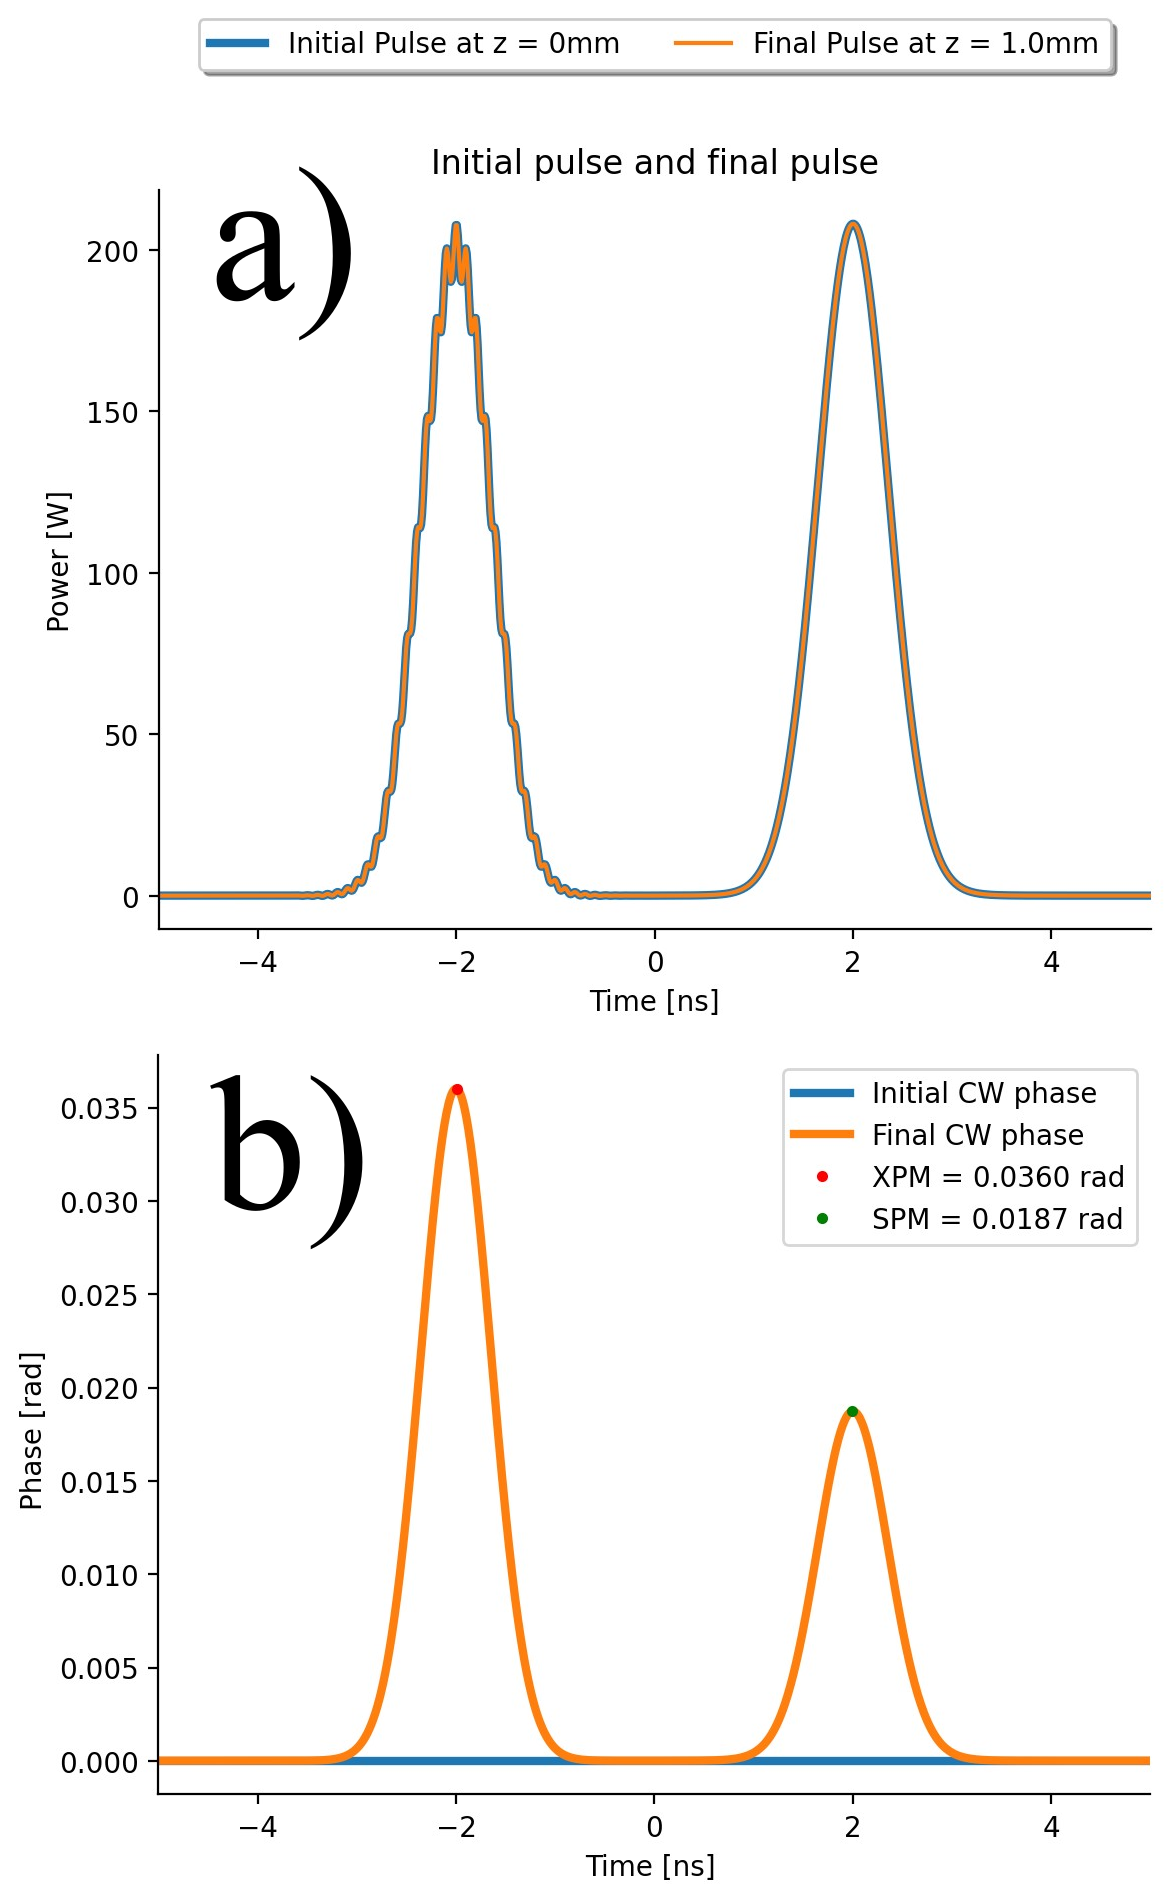
\includegraphics[width=0.8\linewidth]{figures/XPM_combined.png}
    \caption{图示 SPM 和 XPM 对光信号相位的不同影响。 a) 低功率 CW 信号与两个相同的高功率高斯脉冲重叠的时域表示,这两个脉冲的载波频率仅有差别。左侧脉冲的载波频率比 CW 光的载波频率低 10~GHz。 b) 模拟在非线性介质中的传播后,CW 光从 XPM 得到的相移大约是 SPM 的两倍,正如公式 ~\ref{eq:XPM} 所预测的那样。$0.0360/0.0187\approx 1.925\neq2$的比率归因于公式 ~\ref{eq:XPM} 中涉及的近似值以及模拟的有限时间分辨率。这些数字是使用 \href{https://colab.research.google.com/drive/1aIRradfOZGN7JYUhbtYJdVzJwAZoYoUe?usp=sharing}{这个交互式笔记本}生成的,我们鼓励读者尝试使用。}
    \label{fig:XPM}
\end{figure}






\section{相位匹配}
\label{sec:Phase_matching}
小节~\ref{subsec:sidebands}中的推导假定色散可以忽略不计,这是小$\omega_d$值和载波频率接近小节~\ref{subsec:ZDF}中解释的零色散频率的情况。在 \href{https://youtu.be/0SXPvO89jto}{本视频教程}中解释了色散对全波调制的影响。事实证明,当 $\betag_2$ 为正值时,FWM 很弱,而当 $\betag_2$ 为负值时,FWM 最为显著。
\begin{align}
\label{eq:phase_matching}
0&=\betag_2\omega_d^2+\gamma(P_a+P_b)    \\ \nonumber
\betag_2&=-\gamma(P_a+P_b)/\omega_d^2<0,    
\end{align}
假设 $\omega_d$ 足够小,使得在方程~\ref{eq:beta_approx} 中 $\beta_2$ 是唯一相关的项。其原因在于,四波混频(FWM)作为一种过程,涉及电磁波之间通过非线性介质的折射率变化进行**相干**的能量传递。简单来说,非线性效应确保了入射电磁波会引起介质中构成微小偶极子的振荡,从而产生新的时间频率。如果这些偶极子振荡的某一时间频率对应的空间频率与另一电磁波的空间频率相同,该电磁波的功率将通过相干叠加随着传播距离增加而增大,如 \href{https://youtu.be/bha8SzWzRc4}{此视频教程} 所解释的那样。

方程~\ref{eq:phase_matching} 的要求源于入射波与新产生波的空间频率差需要很小,同时入射场功率引起的折射率增大使得空间频率比正常情况更大。因此需要负值的 $\beta_2$ 来进行补偿。这种现象,即介质正常折射率引起的空间频率变化与场功率通过非线性引起的空间频率变化达到平衡,被称为“相位匹配”。方程~\ref{eq:phase_matching} 中的相位匹配条件专门针对四波混频的特殊情况,而类似的表达式也可以推导出适用于本教程范围之外的其他非线性效应,例如 \href{https://www.youtube.com/watch?v=UpuN0dS23Nw}{二次谐波生成}、\href{https://youtu.be/bha8SzWzRc4}{三次谐波生成} 以及 \href{https://www.creol.ucf.edu/mir/wp-content/uploads/sites/7/2023/07/L22_-Stimulated-Brillouin-scattering.pdf}{受激布里渊散射}。
\subsection{调制不稳定(MI)}
由于四波混频(FWM)的影响,在某种非线性介质中,如果载波频率对应的 $\beta_2<0$,信号在传播过程中会变得更加噪声化。这是因为载波与电磁场中微小且无处不在的波动之间的干涉会引发 FWM,将光功率从载波转移到相邻频率上,如 \href{https://prefetch.eu/know/concept/modulational-instability/}{此处} 所解释,并在图~\ref{fig:MI} 中进行了说明。这种由相位匹配导致特定噪声频率被优先放大的过程被称为“调制不稳定性”(Modulation Instability, MI)。关于 MI 的更多细节,请参见 \href{https://youtu.be/VtaoPd0Fwj8}{此视频教程}。

\begin{figure}
    \centering
    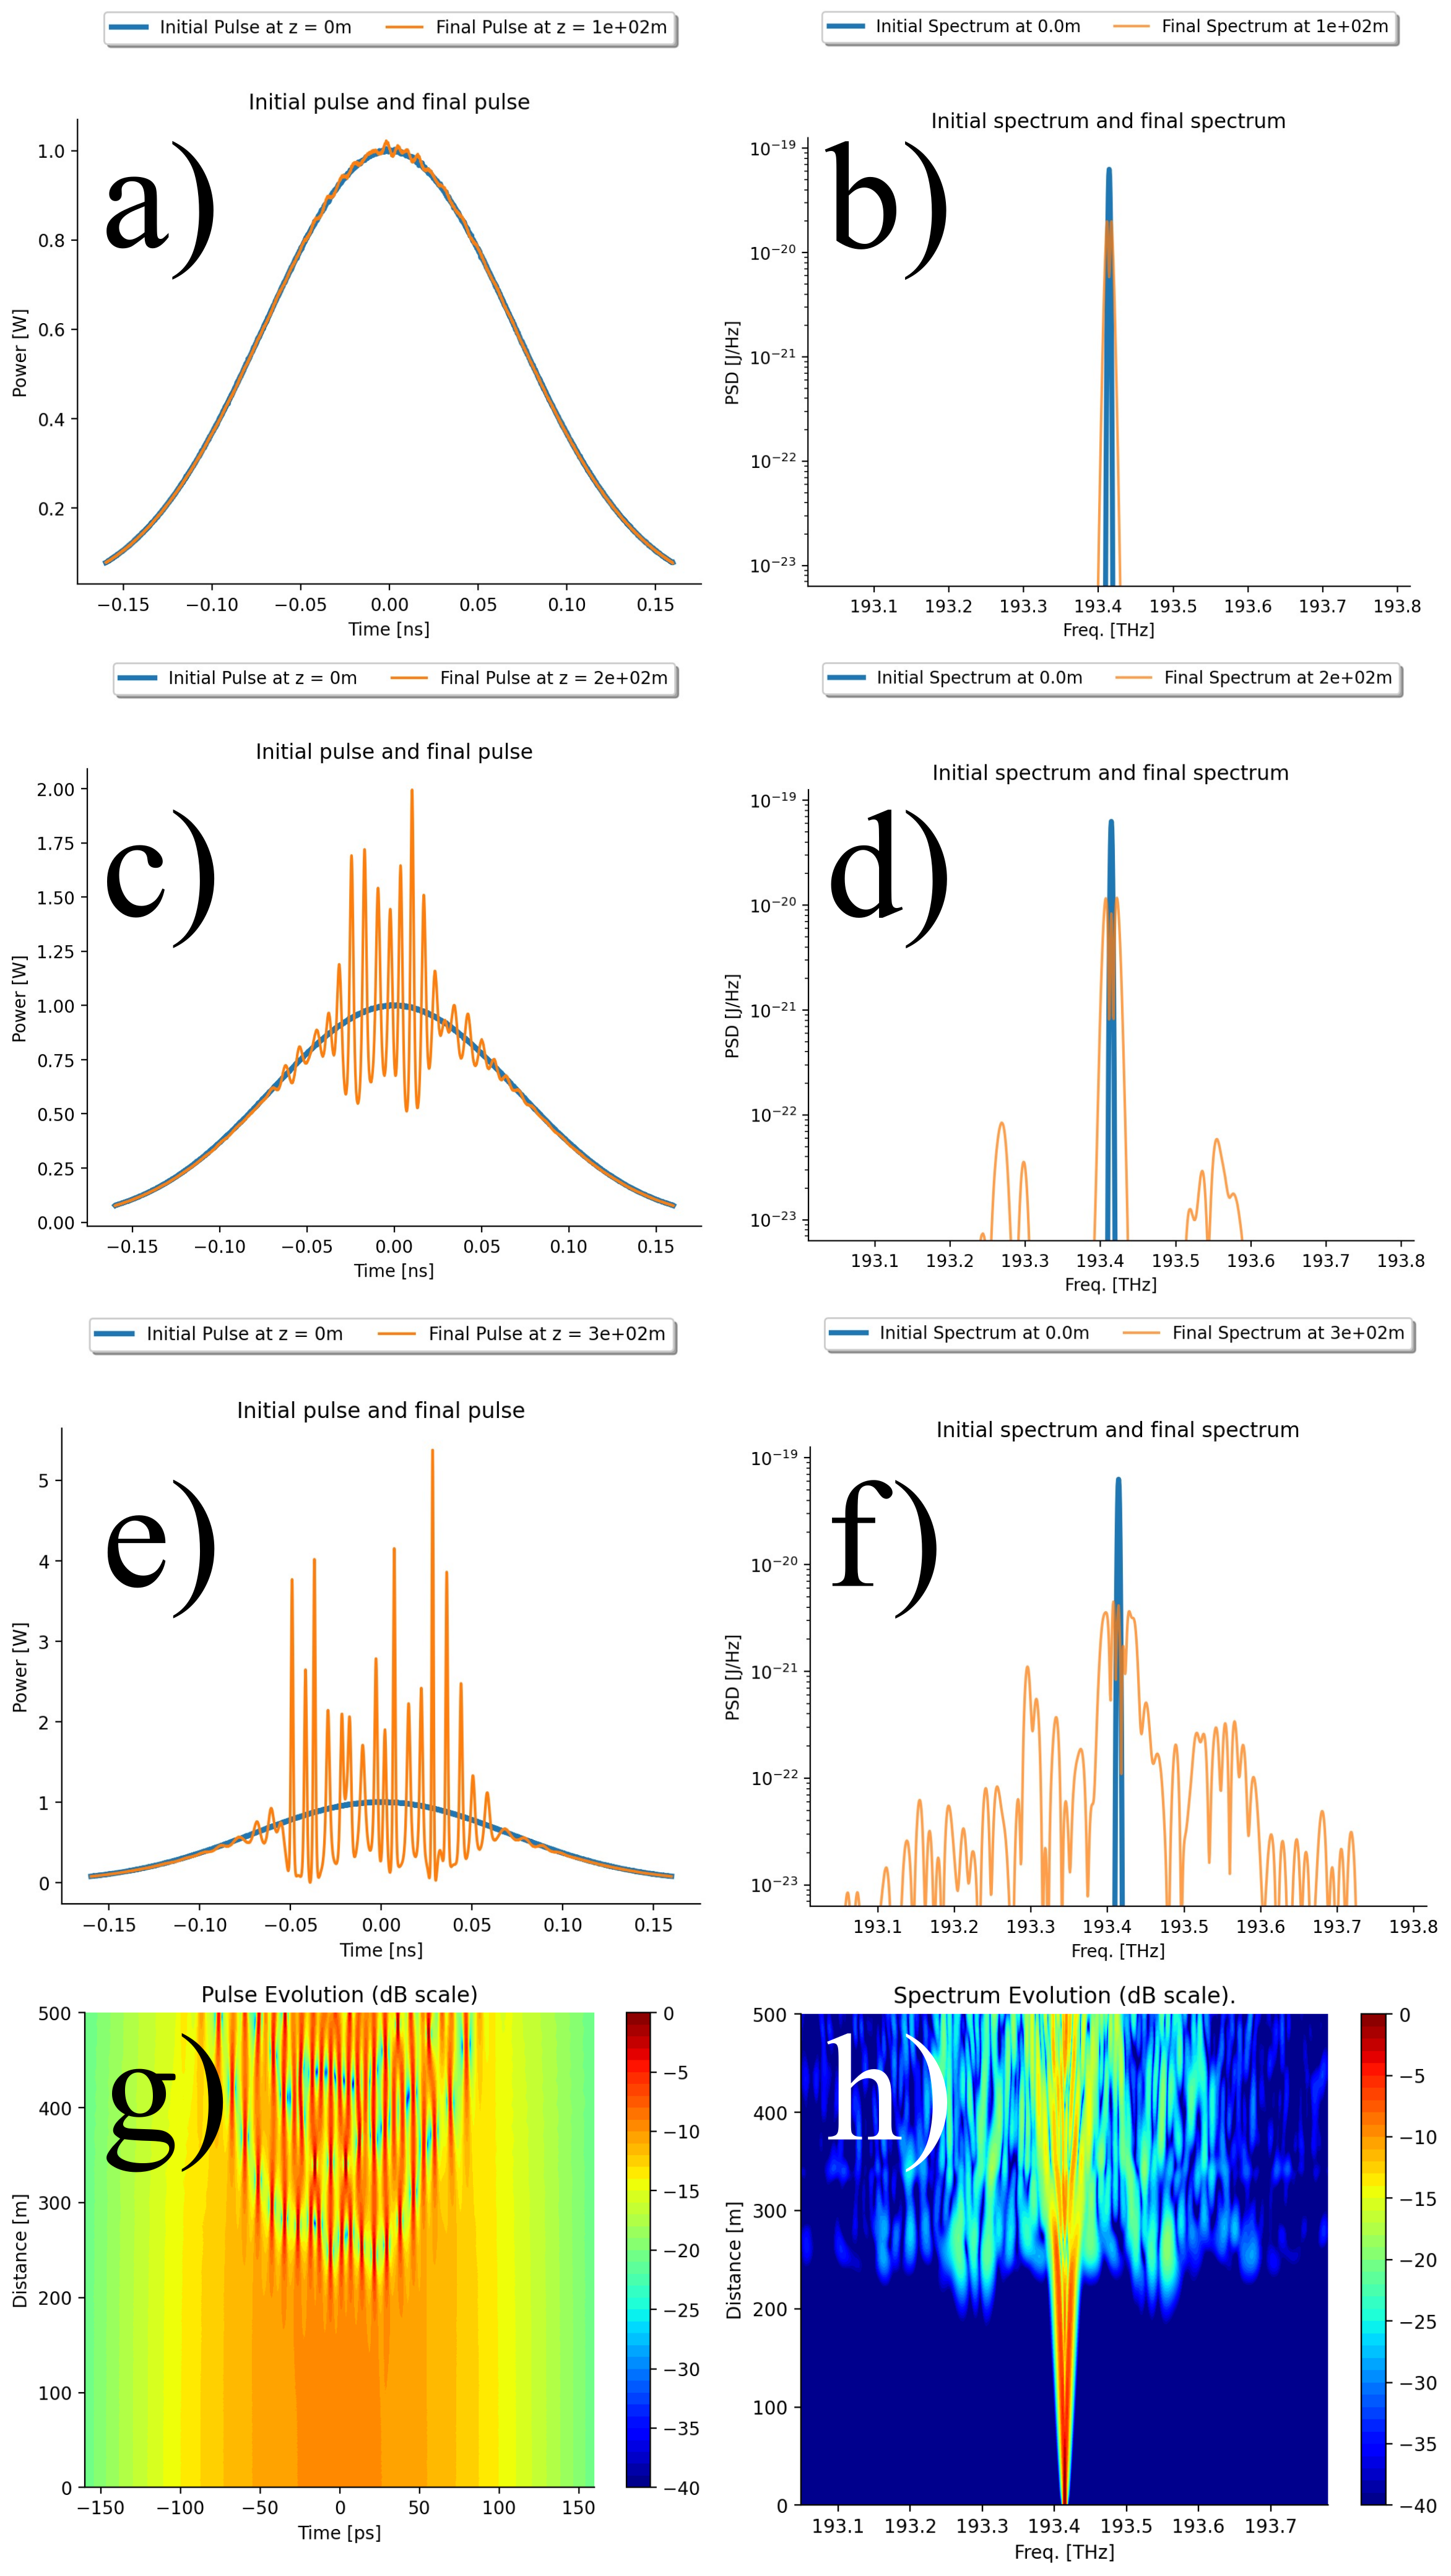
\includegraphics[width=0.75\linewidth]{figures/MI_combined.png}
    \caption{a) 初始和最终时间域信号功率:信号由高斯脉冲和幅度比高斯脉冲小 1.000 倍的随机噪声组成,通过具有 $\beta_2<0$ 的非线性介质传播 100m 后的情况。b) 与 a) 相同,但展示频谱。c-d) 与 a-b) 相同,但传播距离为 200m。e-f) 与 a-b) 相同,但传播距离为 300m。g) 信号在传播 500m 内的完整时间演化。h) 与 g) 相同,但展示频谱。图像由 \href{https://colab.research.google.com/drive/1p2aQZ4zPPAIMplVxvlezdmpQt_j-rsY7?usp=sharing}{此交互式笔记本} 生成,读者可以尝试使用该笔记本进行实验。}
    \label{fig:MI}
\end{figure}



